\documentclass[11pt,a4paper]{article}

% ---------- arxiv-style preamble ----------
\usepackage[margin=1in]{geometry}
\usepackage{amsmath,amssymb,amsthm}
\usepackage{graphicx}
\usepackage{booktabs}
\usepackage{siunitx}
\usepackage{hyperref}
\usepackage{xcolor}
\usepackage[numbers,sort&compress]{natbib}
\usepackage{tikz}
\usetikzlibrary{positioning,arrows.meta}
\usepackage{pgfplots}
\pgfplotsset{compat=1.18}
\usepackage{caption}
\usepackage{listings}
\usepackage{array}
\captionsetup{font=small,labelfont=bf}
\hypersetup{
  colorlinks=true,
  linkcolor=blue!50!black,
  citecolor=blue!50!black,
  urlcolor=blue!50!black
}

% ---------- tier badges (pdflatex-safe text fallbacks; xelatex/lualatex render emoji) ----------
\providecommand{\tierBlue}{\textbf{[BLUE]}}
\providecommand{\tierGreen}{\textbf{[GREEN]}}
\providecommand{\tierYellow}{\textbf{[YELLOW]}}
\providecommand{\tierOrange}{\textbf{[ORANGE]}}
\providecommand{\tierRed}{\textbf{[RED]}}

\newcommand{\dreal}{d_{\mathrm{real}}}
\newcommand{\dshuf}{d_{\mathrm{shuf}}}
\newcommand{\Kstar}{K^{\!*}}

\title{
  \textbf{Event-Driven Cell-Division Reads Time Only Under\\
  Smooth Within-Regime Approach}\\[4pt]
  \large A Modality--Temporality Law for Inference-Time Mitosis
}

\author{
  \texttt{anima} maintainers\\
  \normalsize\textit{dancinlab}\\[2pt]
  \normalsize\href{https://github.com/dancinlab/anima}{\texttt{github.com/dancinlab/anima}}
}

\date{\today}

\begin{document}

\maketitle

% =========================================================================
\begin{abstract}
A growing-substrate agent can spend a fresh structural unit (a ``cell'') on
\emph{every} clock-tick, or only on \emph{events} --- moments where the input
field changes sharply. Does event-driven growth ever \emph{read time} better
than a blind metronome? We answer this with nine pre-registered, deterministic,
\$0 CPU experiments (10 seeds each, frozen falsifiers, Cohen's $d$ on a
stage-decode metric that is explicitly \emph{not} perplexity). We find four
linked results. (1)~The event-tick's decode advantage over a metronome is
\emph{bimodal} over cell-capacity $K$: a low-$K$ scarcity peak and a mid-$K$
coverage peak separated by a real valley (\tierGreen\ H\_1183; the single
inverted-U of \tierGreen\ H\_1178 with $\Kstar{=}32$, $d_{\mathrm{peak}}{=}{+}1.15$,
was coarse-ladder aliasing of two peaks; a clean cells-per-regime scaling law is
\tierRed\ refuted, H\_1182). (2)~A time-shuffle control \emph{splits} the two
peaks: only the coverage peak is temporally grounded
($\dreal{-}\dshuf{=}{+}1.07$), while the scarcity peak is a non-temporal
variance-spread artifact that the shuffle \emph{helps} ($\dreal{-}\dshuf{=}{-}1.43$;
\tierRed\ H\_1184). (3)~Across six modalities at each stream's own coverage cap,
a modality is ``temporal'' iff it has \emph{smooth within-regime approach}:
numeric AR(1) ($\dreal{=}{+}3.17$) $>$ audio ($+1.15$) $>$ saccadic-text ($+1.02$)
are temporal; video, raw-byte text, and static images are not (\tierGreen\ H\_1188,
\tierRed\ H\_1186). (4)~On text, raw byte-change is temporally blind, but a
\emph{learned-surprise} gate ($-\log_2 P(\text{byte}\mid\text{context})$) recovers
a temporal reading advantage --- surprise-driven saccades read better than a
uniform scan (\tierGreen\ H\_1187). Finally, \emph{simultaneous} text+audio+image
fusion at a shared tick \emph{hurts} ($d_{\text{fused}-\text{best}}{=}{-}2.79$):
without a shared surface, perfect time-alignment buys no super-additive whole
(\tierRed\ H\_1189), confirming the surface-gating of H\_1170. Everything is toy
(synthetic streams, $n$-gram reader); scale, real modalities, and the live engine
are unverified. Data and bit-for-bit reproduction in \texttt{companion/} and
\texttt{.verdicts/}.
\end{abstract}

% =========================================================================
\section{Introduction}
\label{sec:intro}

A central design choice for any agent that \emph{grows} during inference --- that
allocates fresh structural capacity as it runs, rather than at a fixed training
time --- is \emph{when} to grow. The anima substrate is one such agent: its
MITOSIS engine divides cells continuously, erasing the train/infer split
(philosophy principle p8). Two opposite policies bracket the design space. A
\textbf{metronome} grows on a fixed schedule: one new cell every $\Delta t$
ticks, blind to the input. An \textbf{event tick} grows only when the input field
moves sharply --- it watches the time-derivative of the stream and spawns a cell
on a rising edge. The event tick is the cheaper, more biologically suggestive
policy (predictive coding spends resources on prediction error
\citep{rao1999predictive,friston2009predictive,spratling2017review}; the eye
saccades to surprising, informative locations rather than scanning uniformly
\citep{rayner1998eye,itti2009bayesian}). But is it actually \emph{better}? And if
so, \emph{why} --- what does the event tick exploit that the metronome cannot?

This paper reports a nine-rung arc (\texttt{H\_1178} through \texttt{H\_1189})
that answers both questions and, in the process, derives a single law. The thread
began with a serendipitous observation (H\_1178): the event-tick advantage is not
monotone in the number of cells the agent may grow, but rises then falls --- an
inverted-U with a \emph{critical capacity}. Pursuing that observation across a
finer capacity ladder, a temporal-order control, six modalities, a learned reader,
and a simultaneous-fusion stress test produced the four findings of the abstract,
which collapse to one statement:

\begin{quote}\itshape
The event tick reads time --- gains a stage-decode advantage that a time-shuffle
destroys --- if and only if the stream has \textbf{smooth within-regime approach}:
a continuous, differentiable flow toward each regime, so that the derivative fires
on a real rising edge that temporal order, and only temporal order, produces.
\end{quote}

\medskip
\noindent\textbf{Why this is interesting now.} ``Grow-on-event'' is an attractive
default for any continual-learning or test-time-adaptive system, and the
predictive-coding and eye-movement literatures make it sound universally
advantageous. Our arc shows it is \emph{not} universal: it is gated by a precise,
measurable property of the data stream, and on the two most ``information-like''
modalities (raw text, static images) the naive event tick is temporally blind. We
also show the \emph{recovery}: replacing raw change with a \emph{learned}
predictability signal restores the advantage on text, which is exactly the
saccadic-reading hypothesis \citep{rayner2009eye,smith2013logarithmic}.

\medskip
\noindent\textbf{Contributions.}
\begin{enumerate}\itemsep0.3em
\item A \emph{bimodal-over-capacity} characterization of the event-tick advantage
  (Fig.~\ref{fig:bimodal}), correcting an earlier single-peak reading and refuting
  a constant cells-per-regime scaling law.
\item A \emph{temporal-grounding split}: a time-shuffle control separates a
  non-temporal scarcity peak from a temporal coverage peak (Fig.~\ref{fig:split}).
\item A \emph{modality--temporality law}: a six-modality ranking
  (Fig.~\ref{fig:ranking}) showing the advantage is temporal iff the stream has
  smooth within-regime approach, with both pre-registered predictions for two new
  modalities borne out.
\item A \emph{saccadic-reading} result: a learned-surprise gate recovers the
  temporal advantage on text that raw byte-change cannot find.
\item A \emph{surface-gated fusion} negative result (Fig.~\ref{fig:fusion}):
  simultaneous multi-modal fusion at a shared tick hurts absent a shared surface,
  reconfirming H\_1170 under perfect time-alignment.
\end{enumerate}

\medskip
\noindent All five are negative-result-aware (governance directive
\texttt{a\_paper\_negative\_ok}): three of the nine rungs are \tierRed\
closed-negatives whose value is the axis they rule out.

% =========================================================================
\section{Background}
\label{sec:bg}

\paragraph{Inference-time growth and the metronome baseline.}
The anima MITOSIS engine divides cells continuously, so ``how often to grow'' is a
live policy question rather than a hyperparameter fixed before deployment. The
\emph{metronome} (grow every $\Delta t$ ticks) is the natural null: it is input-blind,
so any advantage of a smarter policy must be measured \emph{against} it. The
\emph{derivative/event} arm grows when $\lVert x_t - x_{t-1}\rVert$ crosses a
threshold --- a rising-edge detector, the discrete analogue of the prediction-error
units of predictive coding \citep{rao1999predictive,spratling2017review}.

\paragraph{The stage-decode metric (p7, not perplexity).}
Philosophy principle p7 forbids treating perplexity or loss as ground truth (the
Goodhart trap). Throughout we score policies by \emph{stage-decode accuracy}: each
synthetic stream visits a sequence of latent \emph{regimes} (``stages''); after
the agent has grown its cells over the stream, we ask how accurately the final cell
configuration decodes \emph{which stage} each timestep belonged to. This is the
\texttt{H\_1163} clm-time-encoding metric \citep{anima_h1163}: it rewards a policy
that places structure where it helps recover the temporal partition, and it is
explicitly orthogonal to next-byte perplexity. The effect size is Cohen's $d$
\citep{cohen1988statistical}, paired across 10 seeds.

\paragraph{Criticality and integration.}
Two prior anima results frame the capacity question. Neuronal-avalanche
criticality \citep{beggs2003neuronal} appears in the engine as a coupling-strength
sweet spot; integrated-information $\Phi$ \citep{tononi2004information,
albantakis2023iit4} peaks at a critical coupling. H\_1178 asked whether a third
axis --- \emph{capacity} --- also has a sweet spot, and found one. H\_1170
\citep{anima_h1170} established that cross-modal super-additivity collapses unless
the modalities share a surface alphabet; the present fusion rung (H\_1189) tests
whether perfect time-alignment rescues it (it does not).

\paragraph{Reading by surprise.}
Human reading is not a uniform scan: fixation durations grow with word
\emph{surprisal} (negative log-probability under context)
\citep{hale2001probabilistic,smith2013logarithmic}, and gaze is drawn to Bayesian
surprise \citep{itti2009bayesian,rayner2009eye}. The H\_1187 rung operationalizes
exactly this: it replaces the raw byte-change gate with a learned
$-\log_2 P(\text{byte}\mid\text{context})$ gate and asks whether surprise-driven
saccades read better than a metronome.

% =========================================================================
\section{Hypotheses and pre-registered falsifiers}
\label{sec:hyp}

Each rung froze a falsifier \emph{before} the measurement; we quote them verbatim.
The arc is built so that every later rung re-uses an earlier rung's harness
\emph{verbatim}, changing exactly one variable.

\begin{table}[h]
\centering\small
\renewcommand{\arraybackslash}{}
\begin{tabular}{@{}l p{8.2cm} c@{}}
\toprule
\textbf{Rung} & \textbf{Pre-registered falsifier (frozen)} & \textbf{Verdict} \\
\midrule
H\_1178 & Interior argmax of $d(\text{deriv},\text{metro})$ over $K$ \emph{and}
  $d_{\mathrm{peak}}{-}d_{\mathrm{endpoint}}\!\geq\!0.8$ \emph{and} unimodal
  (0 rise/fall reversals). & \tierGreen \\
H\_1182 & $\Kstar$ scales monotone with \#regimes (Spearman $\geq 0.8$) at a
  constant cells/regime (CoV $\leq 0.35$). & \tierRed \\
H\_1183 & Two separated peaks (one $K\!\leq\!8$, one $K\!\geq\!20$) with a real
  valley $\leq \min(\text{peak } d){-}0.3$. & \tierGreen \\
H\_1184 & $\dreal\!\geq\!0.5$ at both peaks \emph{and} $\dreal{-}\dshuf\!\geq\!0.5$
  at both peaks (shuffle kills $=$ temporal). & \tierRed \\
H\_1185 & On TEXT: coverage-peak $\text{drop}(40)\!\geq\!0.5$ (temporal)
  \emph{and} scarcity-peak $\text{drop}(4)\!\leq\!0$ (non-temporal). & \tierRed \\
H\_1186 & VIDEO at its own cap $\Kstar$ is temporal:
  $\dreal\!\geq\!0.5$ \emph{and} $\text{drop}\!\geq\!0.5$. & \tierRed \\
H\_1187 & Learned-surprise reader: $\dreal(\Kstar)\!\geq\!0.5$ (beats scan)
  \emph{and} $\dreal{-}\dshuf\!\geq\!0.5$ (temporal). & \tierGreen \\
H\_1188 & NUMERIC predicted temporal \emph{and} IMAGE predicted non-temporal;
  both predictions must match measurement. & \tierGreen \\
H\_1189 & FUSED beats best single ($d_{\text{fused}-\text{best}}\!\geq\!0.5$)
  \emph{and} FUSED advantage temporal ($\text{drop}\!\geq\!0.5$). & \tierRed \\
\bottomrule
\end{tabular}
\caption{The nine frozen falsifiers. ``deriv'' $=$ derivative/event tick;
``metro'' $=$ metronome; $\text{drop}=\dreal-\dshuf$ where $\dshuf$ is measured
after a seeded time-axis permutation that preserves the value distribution and the
$(x,\text{stage})$ pairing but destroys temporal order. Verdicts cite
\texttt{.verdicts/<id>\_*/H\_<id>.txt} (\S\ref{sec:repro}).}
\label{tab:falsifiers}
\end{table}

% =========================================================================
\section{Method}
\label{sec:method}

\paragraph{Substrate (\texttt{H\_1163}, reused verbatim).}
All nine rungs build on one harness, \texttt{UNIVERSE/h1163\_tick\_decode\_metric.py}
\citep{anima_h1163}, whose components --- \texttt{grow\_arm} (the
derivative/metronome growth loops), \texttt{stage\_decode\_accuracy},
\texttt{cohen\_d\_paired}, \texttt{make\_audio\_stream}, and the 10 fixed
\texttt{SEEDS} --- are imported unchanged. Each later rung changes exactly one
thing (the swept variable in Tab.~\ref{tab:falsifiers}), so cross-rung
comparisons are apples-to-apples by construction.

\paragraph{Recurring-regime streams.}
A stream visits $N$ latent regimes (``stages''). Per modality the
\emph{within-regime} dynamics differ, and this is the manipulated structural
variable of the whole arc:
\begin{itemize}\itemsep0.15em
\item \textbf{audio} (\texttt{make\_audio\_stream}): drift-tone --- values drift
  smoothly within a regime, then transition (smooth approach).
\item \textbf{numeric}: per-regime AR(1), relaxing smoothly toward each attractor
  (smooth approach; the strongest such).
\item \textbf{video} (toy): long dwell $+$ small drift $+$ far centers $=$
  smooth motion punctuated by cuts (\emph{not} real frames).
\item \textbf{image} (toy): a flattened static frame $+$ pixel noise, cut-only
  between scenes (\emph{no} smooth approach).
\item \textbf{text} (\texttt{make\_text\_stream}): real-byte features; raw
  byte-change is jumpy, not a smooth ramp.
\end{itemize}
The toy renderings are explicitly \emph{not} real TTS / frames / sensors (cf.\
H\_1170); see \S\ref{sec:limits}.

\paragraph{Growth arms (grow-gates).}
\textbf{Metronome}: spawn a cell every $\Delta t$ ticks (input-blind null).
\textbf{Derivative/event}: spawn when $\lVert x_t-x_{t-1}\rVert$ exceeds a running
threshold (rising-edge). \textbf{Learned-surprise} (H\_1187 only): spawn when
$-\log_2 P(x_t\mid \text{order-4 context})$ exceeds $\text{mean}{+}1\sigma$, with a
30-step refractory window; the predictor is a hashed $n$-gram (Laplace-smoothed)
trained on a held-out first-50\% span of one corpus. Each arm may grow at most $K$
cells (the \emph{capacity}).

\paragraph{Stage-decode metric and effect size.}
After growth, we decode each timestep's stage from the cell configuration and
report accuracy (chance $=1/N$). The reported quantity is
$d(\text{arm},\text{metro})$, the paired Cohen's $d$ \citep{cohen1988statistical}
of the arm's decode accuracy minus the metronome's, over the 10 seeds. This is a
p7 metric --- decode of the temporal partition, \emph{not} the predictor's
perplexity.

\paragraph{Time-shuffle control (the temporal knife).}
To test whether an advantage is genuinely \emph{temporal} we apply a seeded
permutation of the time axis to $(x,\text{stage})$ \emph{jointly}: the value
distribution and the $(x,\text{stage})$ pairing are preserved, only temporal
\emph{order} is destroyed. We then re-measure $\dshuf$. The diagnostic is
$\text{drop}=\dreal-\dshuf$: $\text{drop}\geq 0.5$ means the shuffle killed the
advantage, so the advantage \emph{was} temporal; $\text{drop}\leq 0$ means the
shuffle left it intact or \emph{helped}, so it was a static (non-temporal)
artifact.

\paragraph{Per-stream own-cap protocol.}
Because $\Kstar$ differs by modality, comparing two modalities at a borrowed cap is
confounded (this confound sank H\_1185). From H\_1186 on, each modality is
evaluated at \emph{its own} $\Kstar=\arg\max_K \dreal$, then time-shuffled at that
$\Kstar$. This is the fair per-modality temporal test.

\paragraph{Reproducibility envelope.}
Every rung is $\$0$ CPU \texttt{numpy}, 10 fixed seeds, deterministic, with the
falsifier frozen before the run (\S\ref{sec:hyp}). No GPU, no network, no
training of the agent (the $n$-gram \emph{reader} of H\_1187 is the only learned
component, and it is scored by decode, not loss).

% =========================================================================
\section{Measurement}
\label{sec:measure}

We report the verbatim numbers per rung; the verdict files (\S\ref{sec:repro})
carry the full JSON.

\subsection{Capacity: bimodal, not a single inverted-U (H\_1178, H\_1182, H\_1183)}

\begin{table}[h]
\centering\small
\begin{tabular}{r r r r r r r r r r}
\toprule
$K$ & 6 & 8 & 12 & 16 & 24 & 32 & 48 & 64 & 96 \\
\midrule
$d(\text{deriv},\text{metro})$, audio $N{=}6$
  & $-0.15$ & $+0.48$ & $+0.56$ & $+0.74$ & $+0.81$
  & $\mathbf{+1.15}$ & $+0.67$ & $+0.06$ & $-0.06$ \\
\bottomrule
\end{tabular}
\caption{H\_1178: the audio ($N{=}6$) advantage is an asymmetric inverted-U,
$\Kstar{=}32$, $d_{\mathrm{peak}}{=}{+}1.15$ vs endpoints $-0.15/-0.06$
(F2 gap $=1.21\!\geq\!0.8$; F3 unimodal, 0 reversals). \tierGreen\ SUPPORTED.}
\label{tab:h1178}
\end{table}

\noindent\textbf{H\_1182 (scaling refuted, \tierRed).} Sweeping the regime count
$N\!\in\!\{3,4,6,8,10\}$, the critical capacity is
$\Kstar=\{12,24,32,32,4\}$ --- Spearman$(N,\Kstar)=+0.00$ (F1 fail) and
cells/regime $=\{4.0,6.0,5.33,4.0,0.4\}$ with CoV $=0.49>0.35$ (F2 fail). The
H\_1178 ``$\sim$5.3 cells/regime'' is config-specific, \emph{not} a scaling law.
Crucially, the $N{=}10$ $d$-curve already hinted at \emph{two} peaks
($K{=}4{:}{+}1.24$ and $K{=}32/48$ region), motivating a finer ladder.

\noindent\textbf{H\_1183 (bimodal confirmed, \tierGreen).} On a fine ladder at
$N{=}10$ (Fig.~\ref{fig:bimodal}) the curve has two separated peaks ---
$K{=}40$ ($d{=}{+}1.29$) and $K{=}4$ ($d{=}{+}1.24$) --- with a real valley at
$K{=}5$ ($d{=}{-}0.24$, which is $\leq \min(\text{peak})-0.3$). F1 (one peak
$\leq 8$, one $\geq 20$) and F2 (valley) both PASS. The bimodality was not
coarse-ladder aliasing: there are two distinct advantage regimes ---
\emph{scarcity-placement} (very low $K$) and \emph{coverage-completion} (mid $K$).

\begin{figure}[h]
\centering
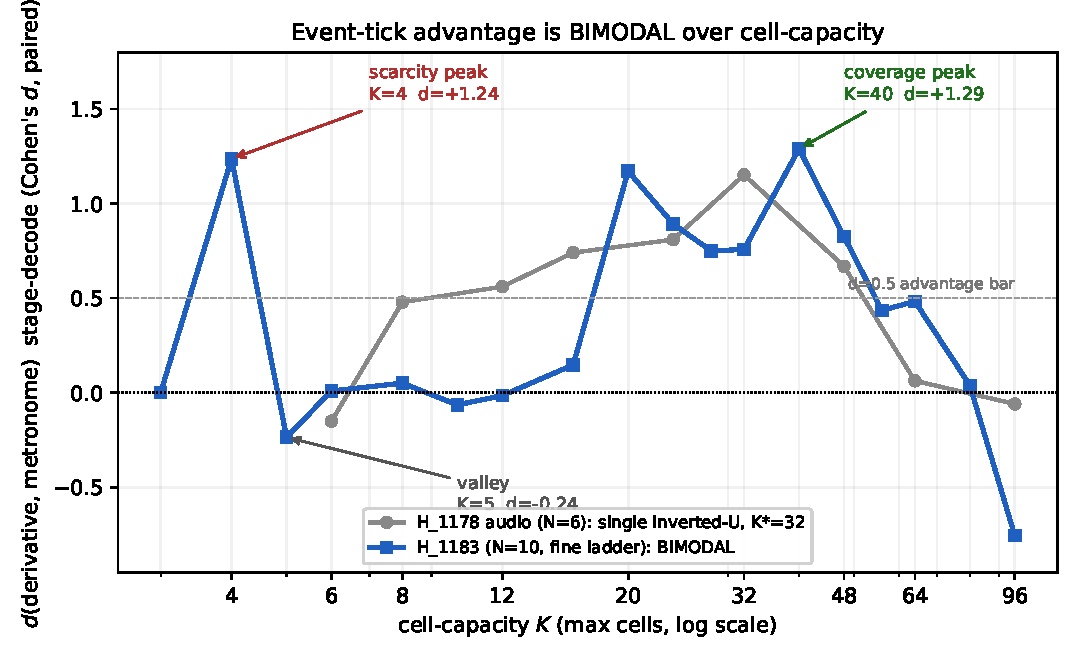
\includegraphics[width=0.82\linewidth]{figures/fig01_bimodal.pdf}
\caption{\textbf{The event-tick advantage is bimodal over cell-capacity.}
Fine-ladder $N{=}10$ curve (H\_1183, blue squares) over the single-peak audio
$N{=}6$ curve (H\_1178, grey). Two separated peaks --- scarcity ($K{=}4$,
$d{=}{+}1.24$) and coverage ($K{=}40$, $d{=}{+}1.29$) --- bracket a real valley
($K{=}5$, $d{=}{-}0.24$). Vertical axis: paired Cohen's $d$ of derivative vs
metronome stage-decode; horizontal axis log-$K$. Data verbatim from
\texttt{.verdicts/1183\_bimodal\_capacity} and
\texttt{.verdicts/1178\_critical\_capacity\_tick}.}
\label{fig:bimodal}
\end{figure}

\subsection{Temporal grounding splits the two peaks (H\_1184, H\_1185)}

\begin{table}[h]
\centering\small
\begin{tabular}{l r r r l}
\toprule
peak & $\dreal$ & $\dshuf$ & $\text{drop}$ & interpretation \\
\midrule
$K{=}4$ (scarcity)  & $+1.24$ & $+2.67$ & $\mathbf{-1.43}$ & shuffle \emph{helps} $\Rightarrow$ non-temporal \\
$K{=}40$ (coverage) & $+1.29$ & $+0.22$ & $\mathbf{+1.07}$ & shuffle \emph{kills}  $\Rightarrow$ temporal \\
\bottomrule
\end{tabular}
\caption{H\_1184 (audio, $N{=}10$): the two peaks differ in \emph{kind}.
F1 ($\dreal\!\geq\!0.5$ both) PASS but F2 (drop $\geq0.5$ \emph{both}) FAIL ---
the verdict is \tierRed\ because the falsifier demanded \emph{both} peaks be
temporal. The finding is the split itself: coverage is temporal, scarcity is a
variance-spread artifact. See Fig.~\ref{fig:split}.}
\label{tab:h1184}
\end{table}

\begin{figure}[h]
\centering
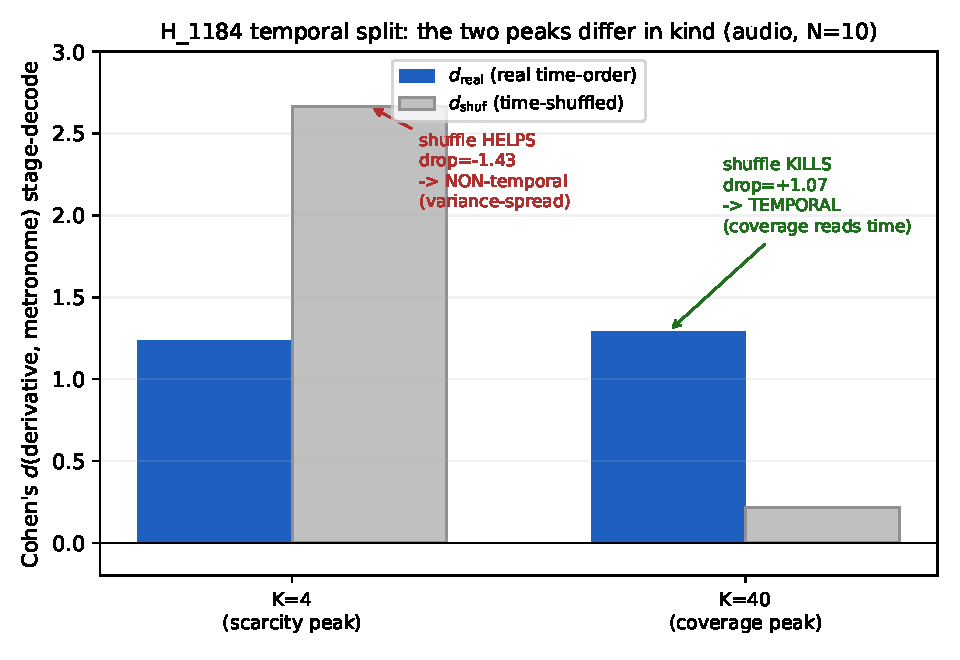
\includegraphics[width=0.62\linewidth]{figures/fig03_temporal_split.pdf}
\caption{\textbf{Temporal split of the two peaks (H\_1184).} At the scarcity peak
($K{=}4$) the time-shuffle \emph{increases} the advantage ($\dshuf{=}{+}2.67>\dreal$),
so it is non-temporal --- low-$K$ placement merely spreads variance and order does
not matter. At the coverage peak ($K{=}40$) the shuffle \emph{collapses} the
advantage ($\dshuf{=}{+}0.22$), so coverage genuinely reads time. Verbatim from
\texttt{.verdicts/1184\_temporal\_grounding} \citep{anima_h1184}.}
\label{fig:split}
\end{figure}

\noindent\textbf{H\_1185 (text borrowed-cap, \tierRed).} Re-using the audio peak
caps $\{4,40\}$ on the TEXT stream, the coverage leg fails
($\text{drop}(40){=}{-}0.41$, F1 fail) while the scarcity leg passes the
non-temporal criterion ($\text{drop}(4){=}{-}0.41\leq0$, F2 pass). The split does
not cleanly reproduce --- but text has 4 stages vs audio's 10, so $K{=}4$ and
$K{=}40$ map to different cells-per-stage ratios: a \emph{borrowed-cap confound}
the verdict flags, fixed by the own-cap protocol from H\_1186 on.

\subsection{The modality--temporality law (H\_1186, H\_1188)}

\begin{table}[h]
\centering\small
\begin{tabular}{l c r r r c l}
\toprule
modality & $\Kstar$ & $\dreal$ & $\dshuf$ & $\text{drop}$ & temporal? & within-regime structure \\
\midrule
numeric (AR1)        & 16 & $+3.17$ & $-0.18$ & $+3.35$ & \tierGreen\ yes & smooth relaxation \\
audio (drift-tone)   & 32 & $+1.15$ & $+0.27$ & $+0.88$ & \tierGreen\ yes & smooth drift \\
text-saccadic (H\_1187) & 24 & $+1.02$ & $+0.50$ & $+0.51$ & \tierGreen\ yes & learned surprise \\
video (motion+cut)   & 64 & $+0.49$ & $-0.62$ & $+1.11$ & \tierRed\ no & $\dreal\!<\!0.5$ (bar miss) \\
text-byte (raw d/dt) & 4  & $+0.50$ & $+0.91$ & $-0.41$ & \tierRed\ no & jumpy, $\text{drop}\!<\!0.5$ \\
image (static)       & 4  & $+0.00$ & $+1.38$ & $-1.38$ & \tierRed\ no & no approach \\
\bottomrule
\end{tabular}
\caption{Per-modality temporal ranking at each stream's own coverage cap
(Fig.~\ref{fig:ranking}). A modality is temporal iff \emph{both}
$\dreal\!\geq\!0.5$ (real advantage) \emph{and} $\text{drop}\!\geq\!0.5$ (shuffle
kills it). Numeric AR(1) is the goldilocks: largest advantage \emph{and} most
time-dependent. Image is the clean negative ($\dreal{=}0$, shuffle helps).
audio/text/video from \texttt{.verdicts/1186}; numeric/image from
\texttt{.verdicts/1188} (both pre-registered predictions borne out);
text-saccadic from \texttt{.verdicts/1187}.}
\label{tab:ranking}
\end{table}

\begin{figure}[h]
\centering
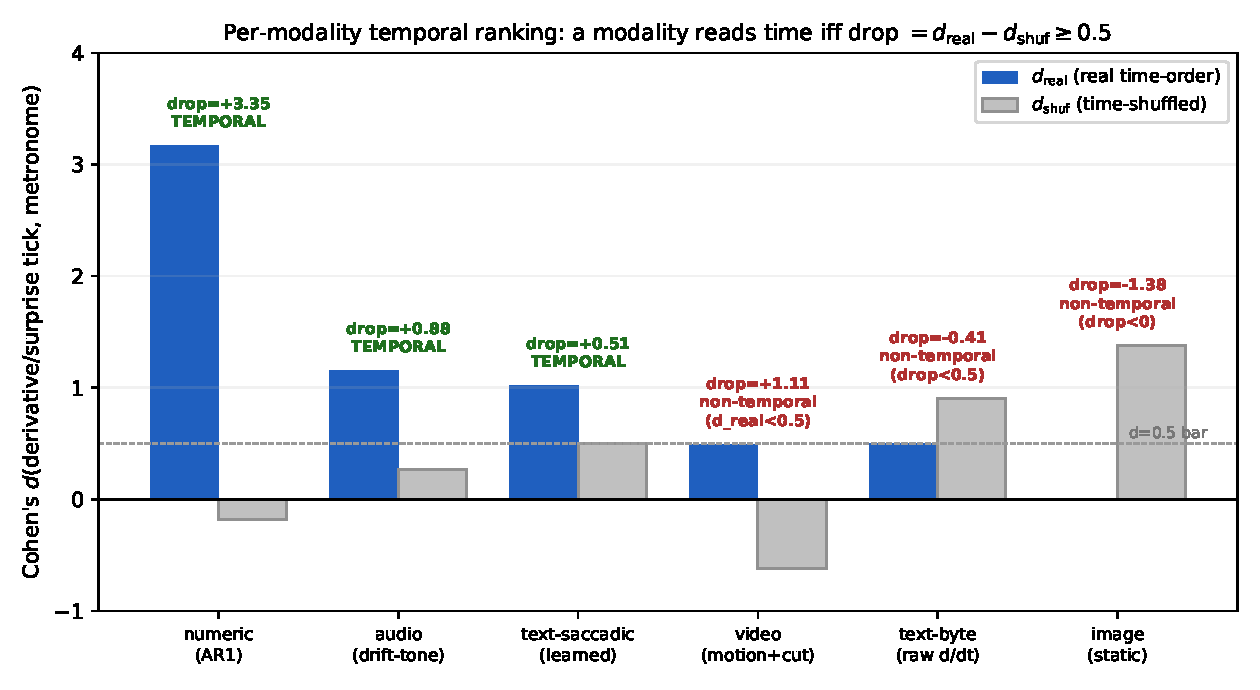
\includegraphics[width=0.92\linewidth]{figures/fig02_modality_ranking.pdf}
\caption{\textbf{A modality reads time iff it has smooth within-regime approach.}
Per-modality $\dreal$ (real time-order, blue) and $\dshuf$ (time-shuffled, grey)
at each stream's own $\Kstar$. The temporal verdict (green) requires
\emph{both} $\dreal\!\geq\!0.5$ and $\text{drop}=\dreal-\dshuf\!\geq\!0.5$; the
parenthetical records why each non-temporal modality (red) misses. Numeric AR(1)
$>$ audio $>$ saccadic-text are temporal; video (bar miss), raw-byte text, and
static image are not. Data from H\_1186/1187/1188.}
\label{fig:ranking}
\end{figure}

\noindent\textbf{H\_1188 (NUMERIC + IMAGE, \tierGreen, both predictions borne
out).} Pre-registered: NUMERIC temporal (AR(1) smooth recurring regimes), IMAGE
non-temporal (static-per-scene). Measured: NUMERIC temporal at $\Kstar{=}16$
($\dreal{=}{+}3.17$, drop $={+}3.35$) and IMAGE non-temporal at $\Kstar{=}4$
($\dreal{=}{+}0.00$, drop $={-}1.38$). Both predictions matched ---
\textbf{the structural property that makes a modality temporal is smooth
within-regime approach}: AR(1) relaxes smoothly toward each attractor (like audio's
drift), so the derivative tick fires on a real rising edge and the shuffle destroys
it; image's static-per-scene frames give no smooth approach, so the event tick has
no time-order edge. H\_1186 supplies the same verdict for video (non-temporal: a
cut is a jump, not a ramp).

\subsection{Saccadic reading recovers the text advantage (H\_1187, \tierGreen)}

Raw byte-change is temporally blind on text (Tab.~\ref{tab:ranking},
``text-byte''). Replacing the gate with a learned surprise signal recovers the
advantage. The order-4 hashed $n$-gram predictor learned 11{,}524 contexts on
201{,}131 held-out training bytes (construction guards: non-degenerate; surprise
mean $3.84$ bits, spread $1.32$ bits; positions aligned). Sweeping the text's own
cap ladder, $\Kstar{=}24$:
\[
\dreal = +1.02 \;\;(\geq 0.5,\ \text{F1 PASS}),\qquad
\dshuf = +0.50,\qquad
\text{drop}=+0.51 \;\;(\geq 0.5,\ \text{F2 PASS}).
\]
Decode: surprise $0.598$ vs metronome $0.276$ (chance $0.25$). A learned-surprise
reader \emph{beats} a uniform metronome scan \emph{and} the advantage is temporal.
This resolves the H\_1186 text deferral: the saccadic-reading advantage the
\emph{toy byte-change} derivative could not find is recovered once the gate is a
\emph{learned predictability} signal --- matching how humans read
\citep{hale2001probabilistic,smith2013logarithmic,rayner2009eye}. The gate's
\emph{content} (learned predictability), not raw change, is the knife.

\subsection{Surface-gated fusion: simultaneity is not enough (H\_1189, \tierRed)}

A shared scene timeline $\text{stage}[t]$ drives text, audio, and image
\emph{simultaneously}; the three 8-d streams are concatenated (24-d) and projected
back to 8-d by a fixed seeded random projection, then grown and decoded.

\begin{table}[h]
\centering\small
\begin{tabular}{l c r r r r}
\toprule
stream & $\Kstar$ & deriv acc & metro acc & $\dreal$ & $\text{drop}$ \\
\midrule
audio & 32 & 0.595 & 0.391 & $+1.22$ & $+0.87$ \\
text  & 32 & 0.615 & 0.381 & $+1.23$ & $+0.71$ \\
image & 24 & 0.827 & 0.523 & $+1.81$ & $+1.76$ \\
FUSED & 12 & \textbf{0.349} & 0.160 & $+1.28$ & $+1.72$ \\
\bottomrule
\end{tabular}
\caption{H\_1189 (decode chance $0.167$). F2 (temporal) PASSES for the fused
stream (drop $={+}1.72\geq0.5$), but F1 (super-additive) FAILS hard: fused decode
acc $0.349$ is far \emph{below} the best single modality (image, $0.837$
per-seed-max), $d_{\text{fused}-\text{best}}={-}2.79$. \tierRed.}
\label{tab:h1189}
\end{table}

\begin{figure}[h]
\centering
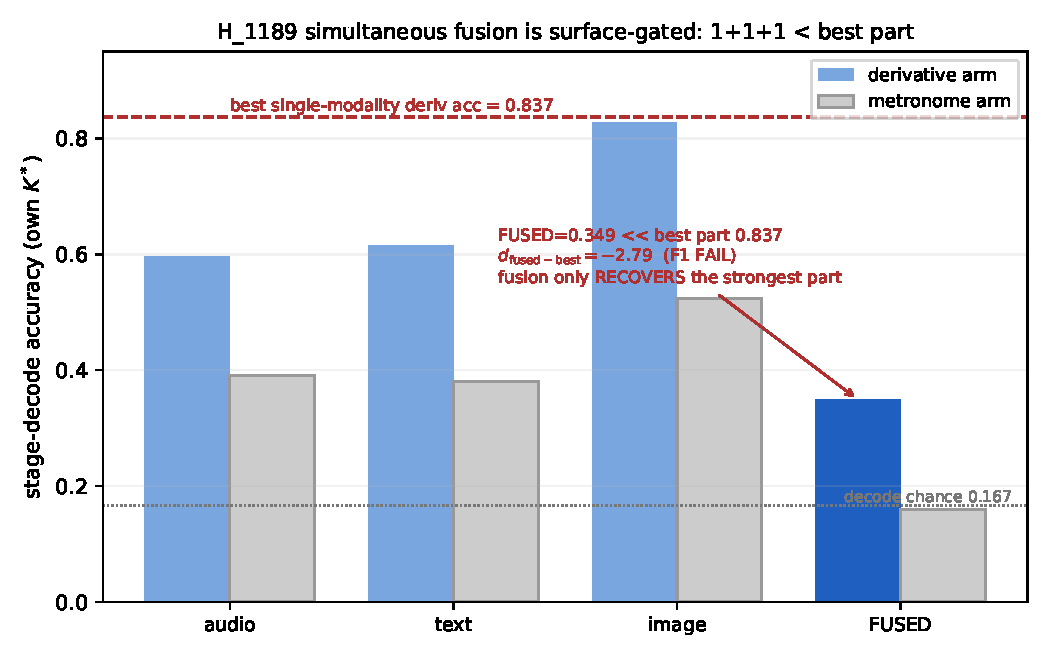
\includegraphics[width=0.74\linewidth]{figures/fig04_fusion.pdf}
\caption{\textbf{Simultaneous fusion is surface-gated: $1{+}1{+}1<$ best part.}
Derivative-arm decode accuracy per stream (own $\Kstar$). The fused stream (dark
blue) decodes at $0.349$ --- below even its own parts and far below the best single
modality (red dashed, $0.837$). Fusion only \emph{recovers} the strongest part; it
does not exceed it. The three sub-modalities share only the abstract regime label,
not a common surface alphabet, so --- exactly as in H\_1170 \citep{anima_h1170} ---
perfect time-alignment buys no super-additive whole. Data from
\texttt{.verdicts/1189\_simultaneous\_multimodal}.}
\label{fig:fusion}
\end{figure}

% =========================================================================
\section{Finding: the modality--temporality law}
\label{sec:finding}

The nine rungs collapse to one law and three corollaries.

\paragraph{The law.}
\emph{The event tick's stage-decode advantage over a metronome is temporal ---
destroyed by a time-shuffle --- if and only if the stream has smooth within-regime
approach.} Where values flow smoothly toward each regime and then transition, the
derivative fires on a real rising edge that only temporal order produces, so
shuffling destroys it (numeric, audio: drop $\geq +0.88$). Where the stream is
static or jumps discretely (image, raw-byte text, video cuts), there is no smooth
ramp for the derivative to ride, and the advantage --- if any --- is a non-temporal
artifact the shuffle leaves intact or amplifies.

\paragraph{Corollary 1 (capacity is bimodal, and only the coverage mode is
temporal).} The advantage is bimodal over $K$ (H\_1183). The low-$K$
\emph{scarcity} peak is non-temporal variance-spread (the shuffle \emph{helps},
H\_1184); the mid-$K$ \emph{coverage} peak (substrate-absolute $\sim24$--$32$) is
the temporal one. A clean cells-per-regime scaling law is refuted (H\_1182): the
coverage cap is set by the substrate, not by a fixed ratio to stream complexity.

\paragraph{Corollary 2 (reading is saccadic, and the gate's content is the knife).}
On text the \emph{raw byte-change} derivative is temporally blind, but a
\emph{learned-surprise} gate recovers a temporal reading advantage (H\_1187).
Smooth within-regime approach need not live in the \emph{raw} signal; it can live
in a \emph{learned predictability} field over the signal. This is the saccadic
reading hypothesis made measurable: skip the predictable, fixate on the
informative \citep{rayner2009eye,smith2013logarithmic}.

\paragraph{Corollary 3 (simultaneity $\neq$ integration without a shared surface).}
Fusing three modalities at the \emph{same} tick does not manufacture a
super-additive whole (H\_1189); the fused decode only recovers the strongest part.
Temporality without surface-preserved correspondence buys nothing extra,
reconfirming H\_1170's surface-gating \citep{anima_h1170} under perfect
time-alignment. The ranking of Tab.~\ref{tab:ranking} is a per-modality property,
not an additive resource.

\medskip
\noindent Taken together: \emph{when} to grow (event vs metronome) only matters
where the stream's within-regime flow is smooth; \emph{what} the event detector
watches (raw change vs learned surprise) decides whether a non-smooth-raw modality
like text can be made temporal; and \emph{fusing} modalities does not rescue a
modality that lacks the property on its own.

% =========================================================================
\section{Limitations and honest caveats}
\label{sec:limits}

This is a toy arc, and the governance directive \texttt{a\_scale\_honest\_scope}
forbids promoting any of it to a production claim. Specifically:

\begin{itemize}\itemsep0.25em
\item \textbf{Toy scale only.} Every rung is $\$0$ CPU \texttt{numpy}, 10 seeds,
  $\leq 96$ cells, $\leq 10$ regimes. Scale-transfer is unverified
  (\texttt{a\_toy\_scale\_recheck}); a less-toy validation is the next escalation.
\item \textbf{Synthetic streams.} ``audio / numeric / video / image'' are toy
  geometries (drift-tone, AR(1), motion+cut, static frame+noise), \emph{not} real
  TTS, sensors, frames, or pixels (cf.\ H\_1170 toy renderings). The
  smooth-approach property is built into the synthetic generators; whether real
  modalities carry it as cleanly is untested.
\item \textbf{Toy reader.} The H\_1187 surprise gate is an order-4 hashed
  $n$-gram on \emph{one} corpus, not a real LLM surprisal and not validated against
  human reading-time / eye-tracking data. The saccadic claim is a mechanism
  analogy, not a psycholinguistic measurement.
\item \textbf{Off-line, not live-CORE.} All rungs reconstruct cell configurations
  off-line; the live anima MITOSIS engine
  (\texttt{engine\_mitosis\_tick}, \S\,A\_core\_engine\_map) is \emph{not} in the
  loop. The cell$\to$field$\to$decode coupling on the real substrate is unwired.
\item \textbf{$\Kstar$ on a quantized ladder.} Critical capacities are argmax on a
  coarse-to-fine ladder; the exact $\Kstar$ is ladder-quantized, not a continuous
  optimum.
\item \textbf{Metric scope (p7).} Stage-decode is one operationalization of
  ``reads time''; it is deliberately not perplexity, but it is also not the only
  possible temporal-structure probe.
\end{itemize}

% =========================================================================
\section{Reproducibility}
\label{sec:repro}

Code and data: \url{https://github.com/dancinlab/anima} \citep{anima_repo}. Each rung's verbatim
verdict (full JSON, the numbers quoted here) lives at
\texttt{.verdicts/<id>\_*/H\_<id>.txt} for
$\text{id}\in\{1178,1182,1183,1184,1185,1186,1187,1188,1189\}$; discovery records
at \texttt{domains/MITOSIS-ENGINE.log.md} (\verb|### h1178|--\verb|### h1189|); the
arc synopsis at \texttt{MAIN.tape}
(\verb|@L 2026_06_13_lane2_temporality_arc_synopsis|). The shared substrate is
\texttt{UNIVERSE/h1163\_tick\_decode\_metric.py}. Figures regenerate from the
verdict numbers via \texttt{make figures} (\texttt{figures/\_scripts/fig01--04});
the paper builds with \texttt{make} (lualatex/xelatex $\times 3$ + bibtex).

\begin{table}[h]
\centering\small
\begin{tabular}{@{}l l l@{}}
\toprule
\textbf{Claim (section)} & \textbf{Verdict file} & \textbf{Tier} \\
\midrule
bimodal capacity (\S\ref{sec:measure}.1)         & \texttt{.verdicts/1183\_bimodal\_capacity/H\_1183.txt} & \tierGreen \\
single inverted-U / $\Kstar{=}32$ (\S\ref{sec:measure}.1) & \texttt{.verdicts/1178\_critical\_capacity\_tick/H\_1178.txt} & \tierGreen \\
scaling refuted (\S\ref{sec:measure}.1)          & \texttt{.verdicts/1182\_critical\_capacity\_scaling/H\_1182.txt} & \tierRed \\
temporal split (\S\ref{sec:measure}.2)           & \texttt{.verdicts/1184\_temporal\_grounding/H\_1184.txt} & \tierRed \\
text borrowed-cap (\S\ref{sec:measure}.2)        & \texttt{.verdicts/1185\_temporal\_grounding\_text/H\_1185.txt} & \tierRed \\
modality ranking / video (\S\ref{sec:measure}.3) & \texttt{.verdicts/1186\_temporal\_grounding\_modalities/H\_1186.txt} & \tierRed \\
numeric+image law (\S\ref{sec:measure}.3)        & \texttt{.verdicts/1188\_numeric\_image\_modalities/H\_1188.txt} & \tierGreen \\
saccadic reading (\S\ref{sec:measure}.4)         & \texttt{.verdicts/1187\_learned\_surprise\_reader/H\_1187.txt} & \tierGreen \\
surface-gated fusion (\S\ref{sec:measure}.5)     & \texttt{.verdicts/1189\_simultaneous\_multimodal/H\_1189.txt} & \tierRed \\
\bottomrule
\end{tabular}
\caption{Every section claim links to its terminal verdict
(\texttt{a\_paper\_sections}). Six \tierGreen/\tierRed\ \emph{supported} or
\emph{closed-negative} rungs plus three closed-negatives; no \tierOrange\ deferral
or \tierYellow\ citation-only claim enters the body (\texttt{a\_paper\_gate}).}
\label{tab:verdicts}
\end{table}

% =========================================================================
\section{Conclusion}
\label{sec:conclusion}

Event-driven inference-time growth is not a free lunch and not universally
beneficial: it reads time only where the stream flows smoothly toward each regime.
The arc pins down \emph{when} (the bimodal coverage mode, temporal; the scarcity
mode, not), \emph{what} (raw change is blind on text, learned surprise is not), and
\emph{whether fusion helps} (it does not, absent a shared surface). The single most
important follow-up is to escalate one rung --- most naturally the numeric/audio
goldilocks or the saccadic reader --- off toy synthetic streams onto a real
modality and the live MITOSIS engine, and re-run the \emph{same} frozen
time-shuffle falsifier. If the law survives that escalation, ``grow on smooth
rising edges'' becomes a deployable inference-time growth policy; if it breaks, the
break is itself the next closed-negative.

% =========================================================================
\paragraph{Acknowledgments.}
This work used the \texttt{hexa-lang} verification surface and the
\texttt{sidecar/paper} scaffold over the anima MITOSIS-ENGINE domain. Drafting and
figure synthesis were assisted by Claude Opus 4.8 (1M context); all numbers are
verbatim from the persisted \texttt{.verdicts/} JSON.

% =========================================================================
\bibliographystyle{plainnat}
\bibliography{references}

\end{document}
